\subsubsection{Cloud Service}

Der Cloud Service wurde wie im Konzept beschrieben umgesetzt.
Er dient dazu, die Konfiguration des Praxisrufsystems persistent zu verwalten und Benachrichtigungen von Mobile Clients entgegenzunehmen.
Empfangene Benachrichtigungen werden gemäss der persistierten Konfiguration über den angebundenen Message Service an Mobile Clients weitergeleitet.

Um diese Aufgaben zu erfüllen, bietet der Cloud Service eine REST Schnittstelle an, welche die benötigten Funktionen zugänglich macht.
Die umgesetzte API ist unter \url{https://www.praxisruf.ch/swagger-ui.html} dokumentiert.
Die zugehörige Open API definition ist zudem zusammen mit dem Quellcode des Cloud Services abgelegt\footnote{Siehe Anhang B}.
Dies Beinhaltet die verfügbaren Endpunkte und das Model welches für Input und Ouput Werte dieser Schnittstelle dienen.

\begin{figure}[h]
    \begin{minipage}[b]{1\textwidth}
        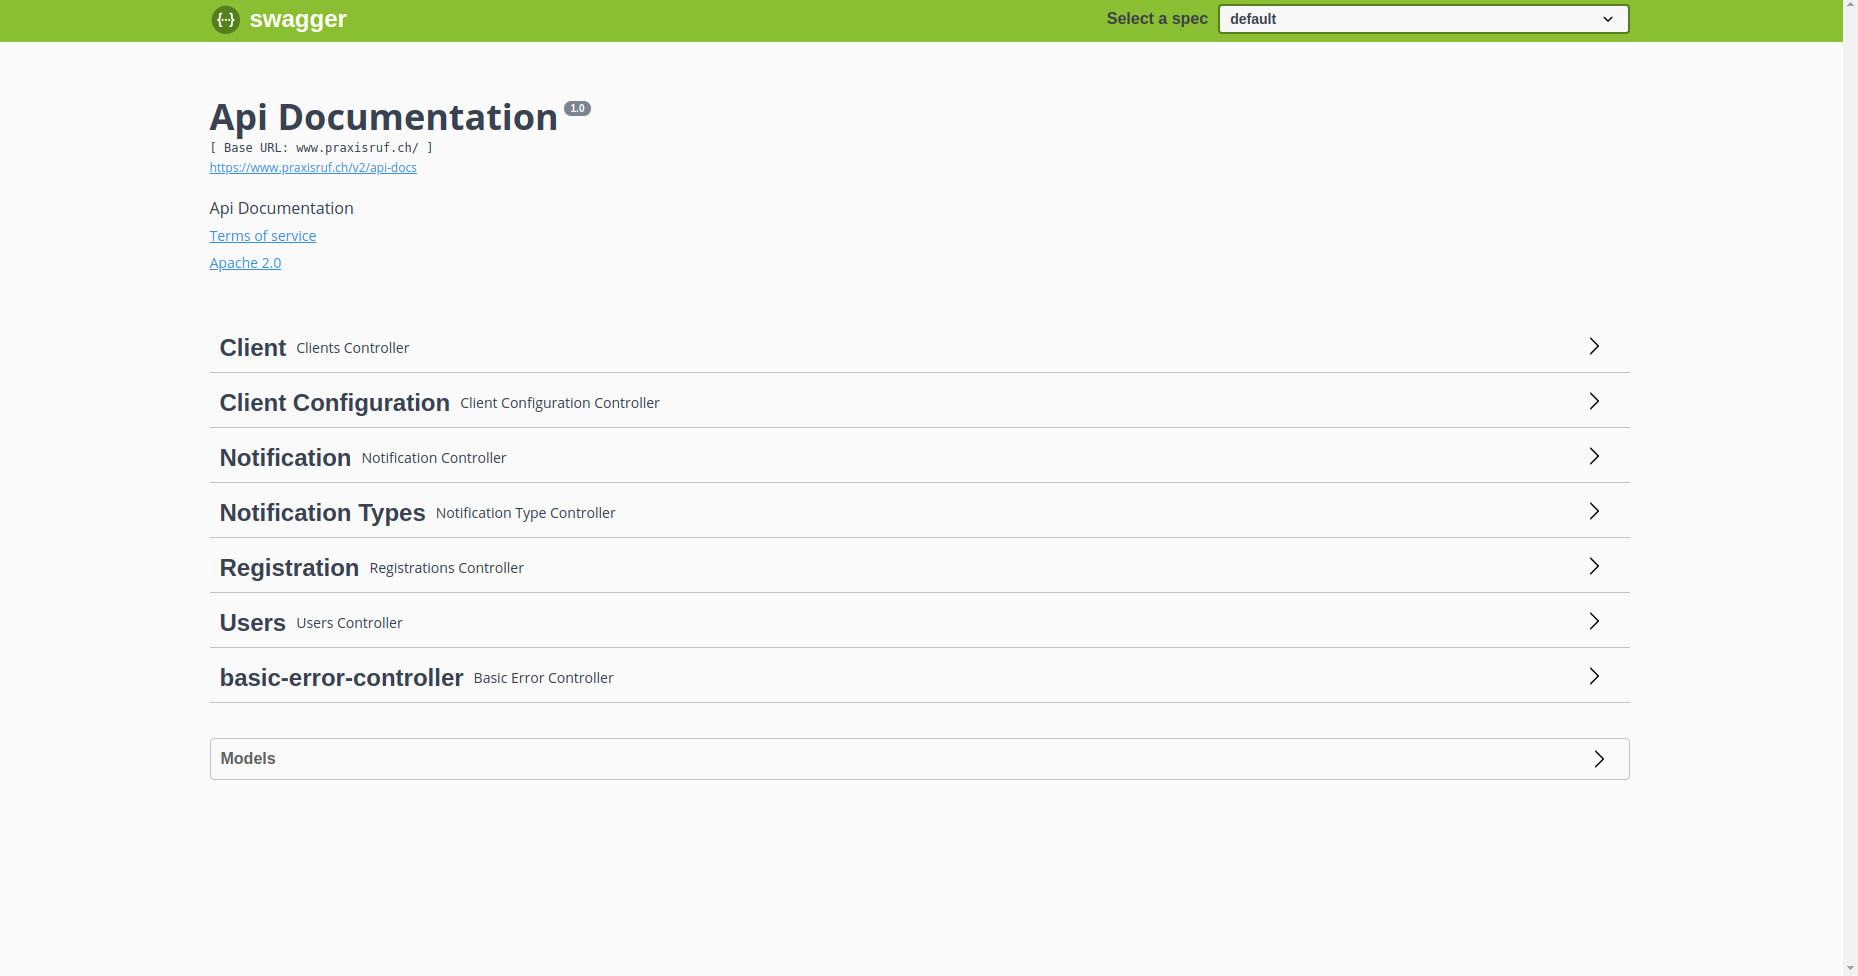
\includegraphics[width=\textwidth]{graphics/screenshots/cloud/swagger-home}
        \caption{Swagger UI}
    \end{minipage}
    \label{fig:swagger}
\end{figure}
\clearpage
